\documentclass{article}
\usepackage[T1]{fontenc}
\usepackage[latin9]{inputenc}
\usepackage{array}
\usepackage{float}
\usepackage{units}
\usepackage{amsmath}
\usepackage{amssymb}
\usepackage[dvips]{graphicx}
\usepackage{tikz}
\usetikzlibrary[arrows,calc,decorations.pathmorphing,backgrounds,positioning,fit,petri,shapes,decorations.markings]
\usepackage{pgfplots}
\newcommand{\lyxdot}{.}


\begin{document}
\begin{figure}
\centering{}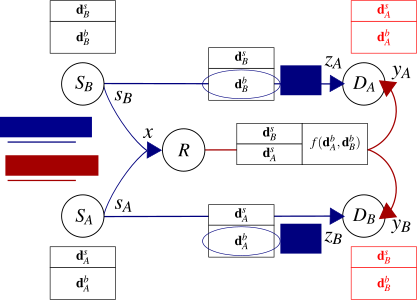
\includegraphics[width=0.6\columnwidth]{fig/2-SRN-sc_principle_BC-TWT_v4}
\caption{Symmetric WBN model with half-duplex constraint and 2-phase communication.\label{fig:CTUpp_Information_flows}}
\end{figure}


\begin{figure*}
\begin{centering}
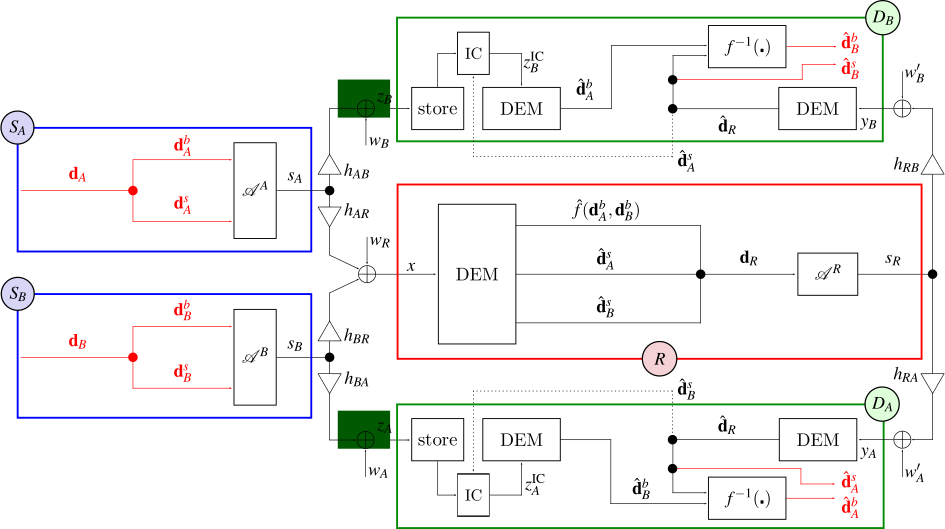
\includegraphics[width=1\textwidth]{fig/butterfly-2level_processing_principleTWC-uncoded}
\par\end{centering}
\caption{Relaying scheme for the uncoded WBN
system. DEM stands for a hard decision demodulator, IC is the interference
canceler.\label{fig:CTUpp_Information-flow-uncoded-block-scheme}}
\end{figure*}


\begin{figure*}
\centering{}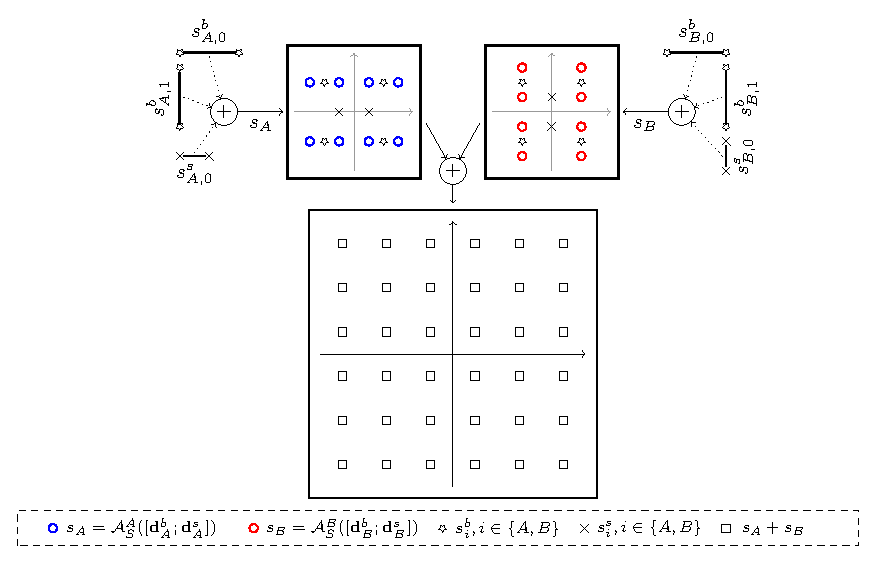
\includegraphics[width=0.8\textwidth]{fig/d2_1}\caption{Source constellation design example for $N_{b}=2,\,N_{s}=1$. Resulting
constellations are depicted as blue circles ($S_{A}$ output constellation),
red circles ($S_{B}$ output constellation) and squares (received
superimposed constellation at $R$). Hierarchical function is $f\left(\mathbf{d}_{A}^{b},\,\mathbf{d}_{B}^{b}\right)=\mathbf{d}_{A}^{b}\oplus\mathbf{d}_{B}^{b}$.\label{fig:CTUpp_ConstellationDesignExample} }
\end{figure*}


\begin{figure*}
\begin{centering}
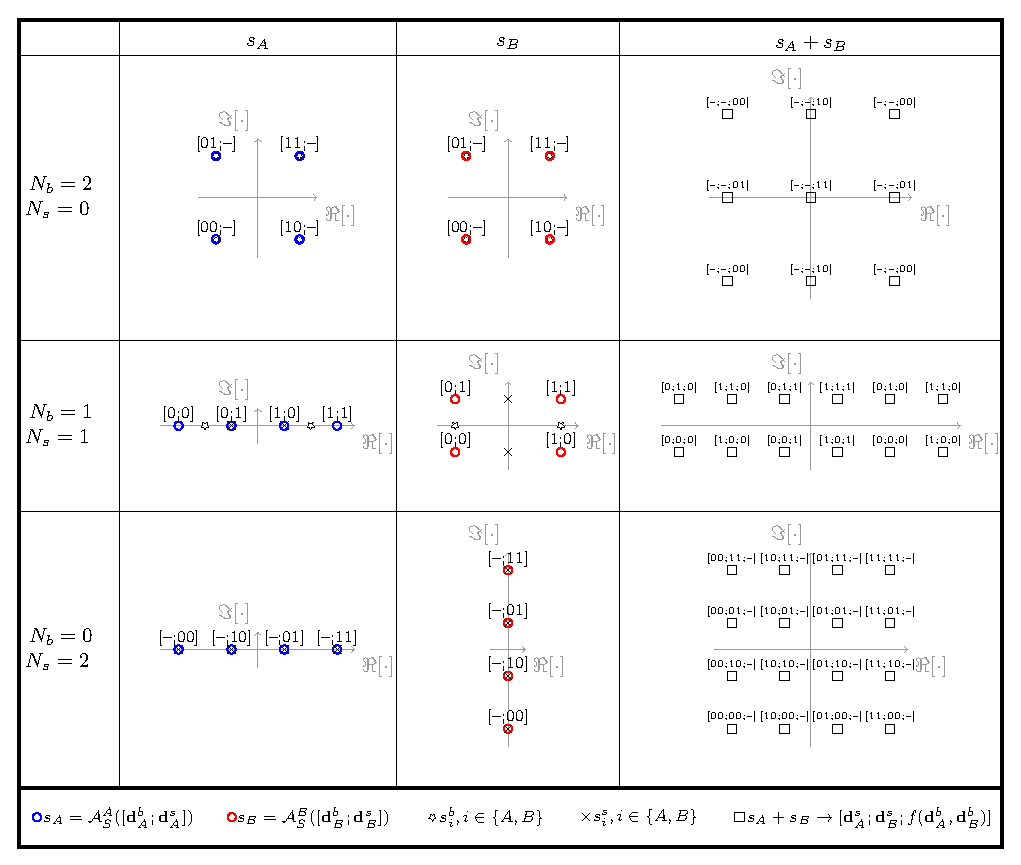
\includegraphics[width=1\textwidth]{fig/const_all_2}
\par\end{centering}

\caption{Proposed constellation design for $\left(N_{b},N_{s}\right)=\left\{ \left(2,0\right);\left(1,1\right);\left(0,2\right)\right\} $.\label{fig:CTUpp_ConstellationDesign_NbNs2} }
\end{figure*}


\begin{figure}
\centering{}\includegraphics[width=0.95\columnwidth]{fig/20150109_143009}\caption{Setup for HW evaluation (Ettus Research
USRPs). Source transmissions are prerotated \cite{Koike-Popovski-Tarokh_2009a,Zhang-Liew_2010,Anxin-Yuan-Kayama_2008}
to imitate the AWGN channel conditions (as used in the numerical evaluation).
To allow a strict control of HSI channels SNR in the HW
setup, the HSI channels are emulated by adding a Gaussian noise to
the respective source signal and the resulting emulated HSI is passed
to destinations via UDP. This also avoids the problem of node visibility
where direct links $S_{A}\rightarrow D_{A}$ and $S_{B}\rightarrow D_{B}$
exist in the laboratory environment.\label{fig:CTUpp_HW_setup}}
\end{figure}


\begin{figure}
\begin{centering}
\hspace*{-0.04\columnwidth}\includegraphics[width=0.95\columnwidth]{fig/Throughput_HSI_XOR_MAC16_BC20_N2}
\par\end{centering}

\caption{Comparison of throughput as a function of $\gamma_{{\rm {HSI}}}$
for $\gamma_{{\rm {MAC}}}=16\,\mathrm{dB},\,\gamma_{{\rm {BC}}}=20\,\mathrm{dB}$
and given $(N_{b},N_{s})$. \label{fig:CTUpp_Throughput16_20}}
\end{figure}


\begin{figure}
\begin{centering}
\hspace*{-0.04\columnwidth}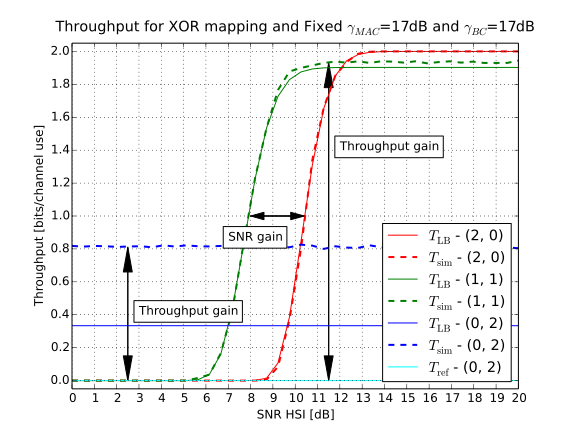
\includegraphics[width=0.95\columnwidth]{fig/Throughput_HSI_XOR_MAC17_BC17_N2}
\par\end{centering}

\caption{Comparison of throughput as a function of $\gamma_{{\rm {HSI}}}$
for $\gamma_{{\rm {MAC}}}=17\,\mathrm{dB},\,\gamma_{{\rm {BC}}}=17\,\mathrm{dB}$
and given $(N_{b},N_{s})$.\label{fig:CTUpp_Throughput17_17}}
\end{figure}


\begin{figure}
\begin{centering}
\hspace*{-0.04\columnwidth}\includegraphics[width=0.95\columnwidth]{fig/Throughput_HSI_XOR_MAC20_BC20_N2}
\par\end{centering}

\caption{Comparison of throughput as a function of $\gamma_{{\rm {HSI}}}$
for $\gamma_{{\rm {MAC}}}=20\,\mathrm{dB},\,\gamma_{{\rm {BC}}}=20\,\mathrm{dB}$
and given $(N_{b},N_{s})$. \label{fig:CTUpp_Throughput20_20}}
\end{figure}


\begin{figure}
\begin{centering}
\hspace*{-0.04\columnwidth}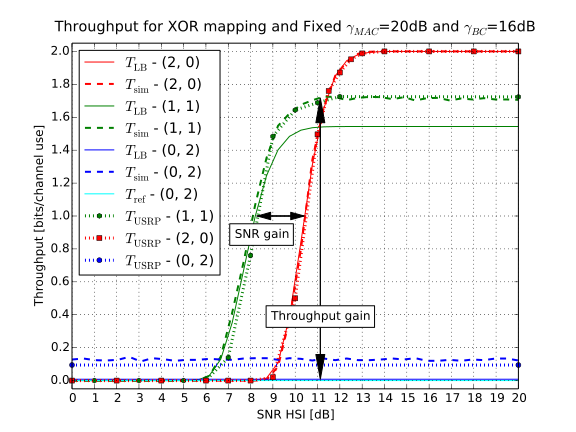
\includegraphics[clip,width=0.95\columnwidth]{fig/Throughput_HSI_XOR_MAC20_BC16_N2}
\par\end{centering}

\caption{Comparison of throughput as a function of $\gamma_{{\rm {HSI}}}$
for $\gamma_{{\rm {MAC}}}=20\,\mathrm{dB},\,\gamma_{{\rm {BC}}}=16\,\mathrm{dB}$
and given $(N_{b},N_{s})$. \label{fig:CTUpp_Throughput20_16}}
\end{figure}


\begin{figure*}
\begin{centering}
\includegraphics[width=0.45\textwidth]{fig/XOR_map_Througput_BC15}\quad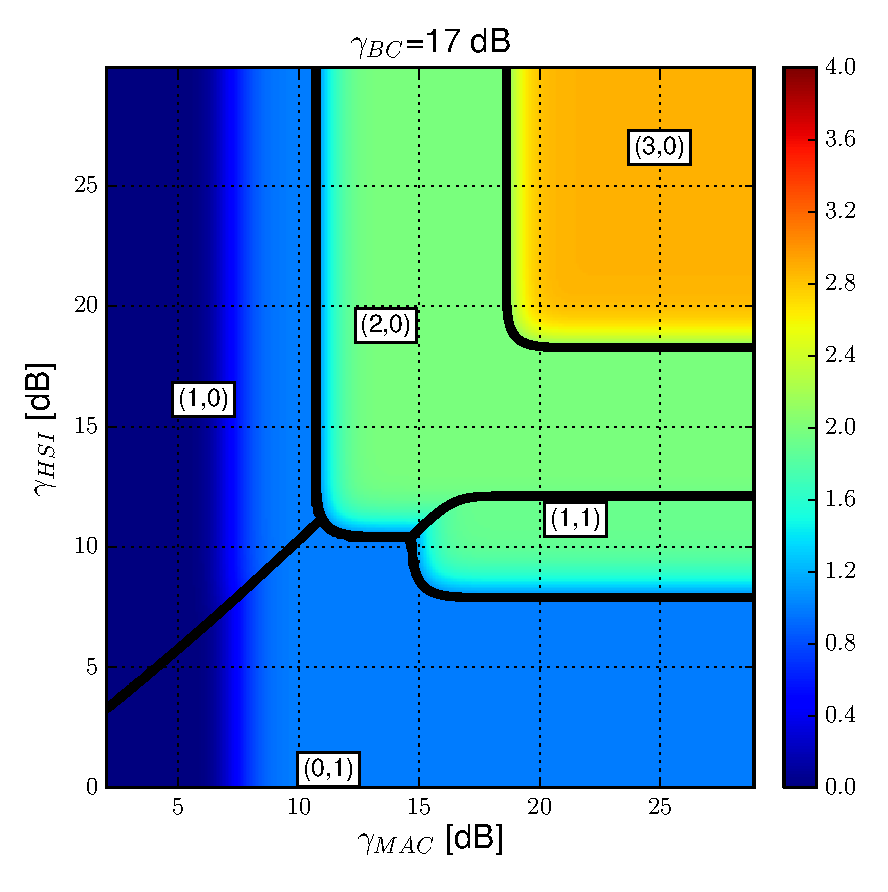
\includegraphics[width=0.45\textwidth]{fig/XOR_map_Througput_BC17}
\par\end{centering}

\centering{}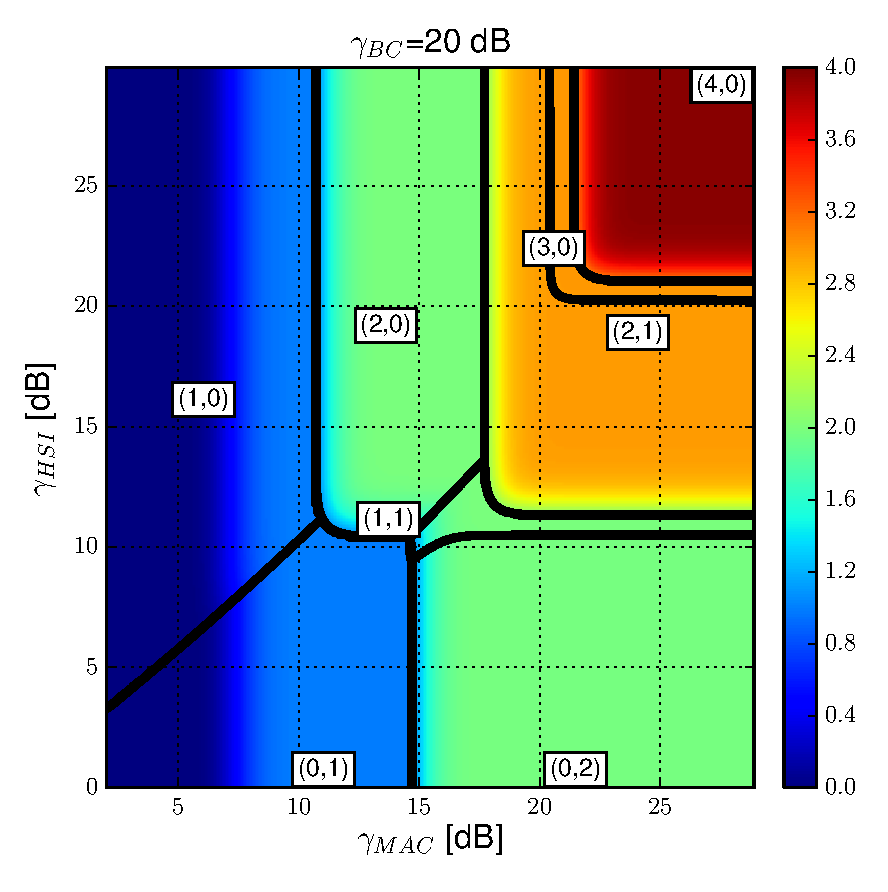
\includegraphics[width=0.45\textwidth]{fig/XOR_map_Througput_BC20}\quad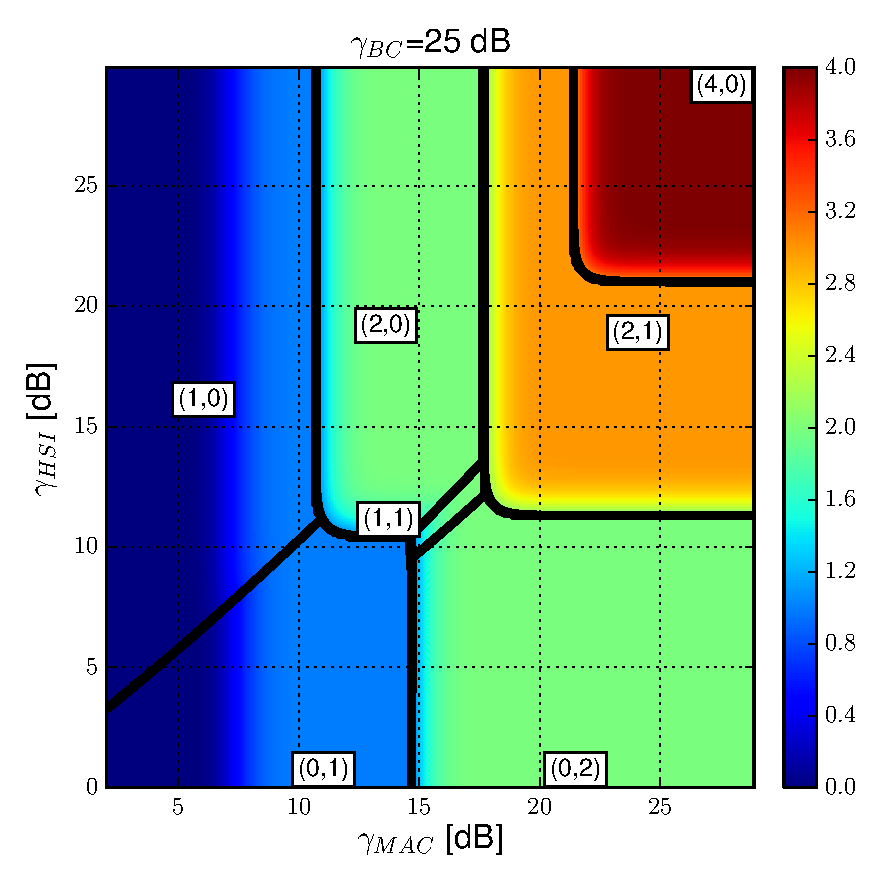
\includegraphics[width=0.45\textwidth]{fig/XOR_map_Througput_BC25}\caption{Throughput performance $T_{\mathrm{LB}}$ and SNR mapping regions
(including the optimal const. parameters ($N_{b}^{{\rm I}},\,N_{s}^{{\rm I}}$))
for $\gamma_{{\rm {BC}}}\in\{15\,\mathrm{dB},\,17\,\mathrm{dB},20\,\mathrm{dB},25\,\mathrm{dB}\}$.\label{fig:CTUpp_SNR_map_BC15-17-20-25}}
\end{figure*}


\begin{figure*}
\centering{}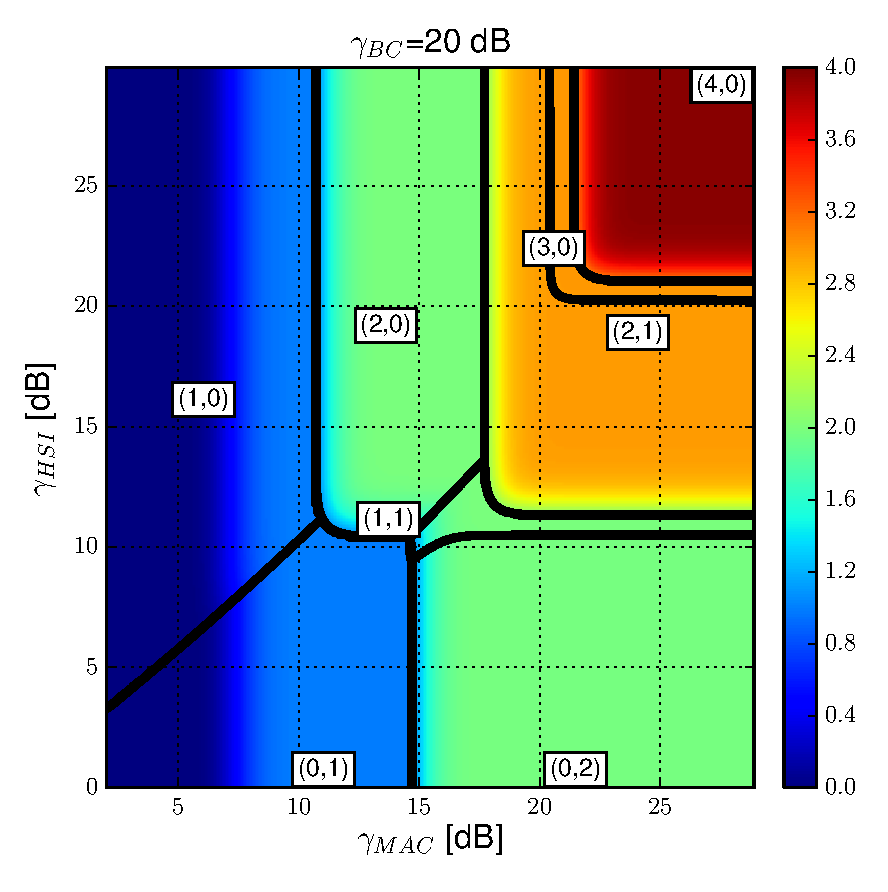
\includegraphics[width=0.48\textwidth]{fig/XOR_map_Througput_BC20}\quad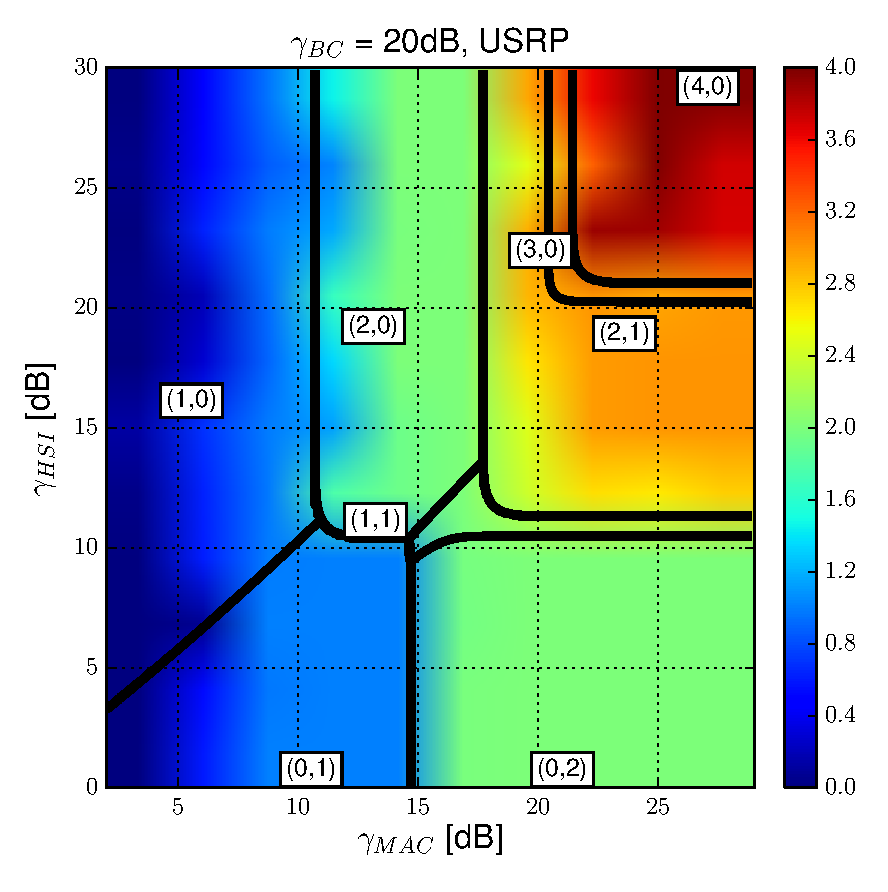
\includegraphics[width=0.48\textwidth]{fig/XOR_map_Througput_USRP_BC20}\caption{Comparison of $T_{\mathrm{LB}}$ and the throughput performance evaluated
in a real world adaptive HW setup ($T_{\mathrm{USRP}}$) for $\gamma_{{\rm {BC}}}=20\,\mathrm{dB}$.
The SNR mapping regions (including the optimal const. parameters ($N_{b}^{{\rm I}},\,N_{s}^{{\rm I}}$))
used in the HW evaluation are also emphasized in the figure.\label{fig:CTUpp_SNR_map_BC20_USRP}}
\vspace*{-4ex}
\end{figure*}


\begin{figure*}
\begin{centering}
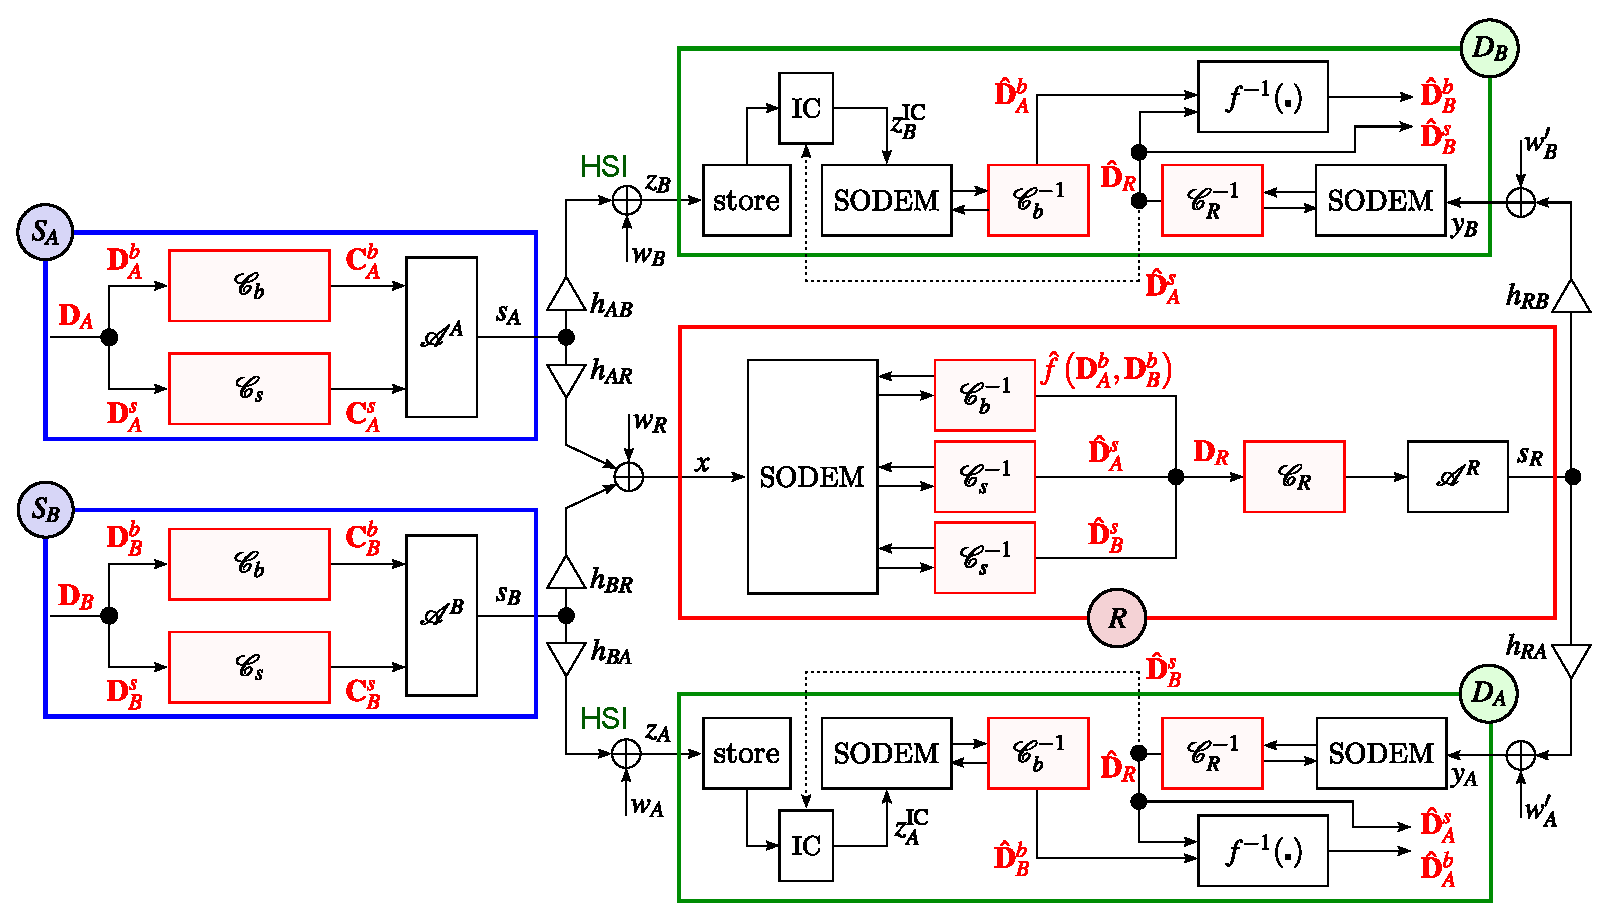
\includegraphics[width=1\textwidth]{fig/butterfly-2level_processing_principleTWC-coded}
\par\end{centering}

\caption{Relaying scheme in the encoded WBN system. SODEM stands for a soft-output
demodulator, IC is the interference canceler. The channel encoders/decoders
which are appended to the uncoded system are emphasized. \label{fig:CTUpp_Information-flow-coded-block-scheme}}
\vspace*{-3ex}
\end{figure*}


\begin{figure*}
\begin{centering}
\hspace*{-1.5em}\includegraphics[width=0.7\columnwidth]{fig/Rate_Regions_XOR_map_BC10_MAC12_HSI8}
\par\end{centering}

\begin{centering}
\includegraphics[width=0.7\textwidth]{fig/Rate_Regions_XOR_map_BC5_MAC5_HSI0}
\par\end{centering}

\caption{Numerically evaluated cut-set bounds (mutual information for finite
input constellations) for $(N_{b}=2,N_{s}=1)$ source constellations
and $16$-QAM at the relay. The particular SNR conditions are available
in the titles of both sub-figures.\label{fig:CTUpp_CSB_eval}}
\end{figure*}


\begin{figure*}
\centering{}\includegraphics[width=0.45\textwidth]{fig/Adaptive_Maps_overall_BC_7\lyxdot 5}~~~\includegraphics[width=0.45\textwidth]{fig/Adaptive_Maps_overall_BC_15\lyxdot 0}\caption{Maximal encoded system throughput $T_{C}^{\mathrm{max}}$ for $\gamma_{{\rm {BC}}}=7.5\,\mathrm{dB}$
and $\gamma_{{\rm {BC}}}=15\,\mathrm{dB}$.\label{fig:CTUpp_Coded_SNR_map} }
\end{figure*}


\begin{figure*}
\centering{}\includegraphics[width=0.45\textwidth]{fig/XOR_map_Througput_coding_Gain7\lyxdot 5}~~~\includegraphics[width=0.45\textwidth]{fig/XOR_map_Througput_coding_Gain15\lyxdot 0}\caption{Throughput enhancement $\Delta T_{C}=T_{C}^{\mathrm{max}}-T_{\mathrm{LB}}$
{[}bits/channel use{]} of the coded over uncoded WBN system for $\gamma_{{\rm {BC}}}=7.5\,\mathrm{dB}$
and $\gamma_{{\rm {BC}}}=15\,\mathrm{dB}$. Note that $0.75\leq\Delta T_{C}\leq2$
in the analyzed range of channel SNRs.\label{fig:CTUpp_Coded_ThroughputGain}}
\end{figure*}


\begin{figure}
\begin{centering}
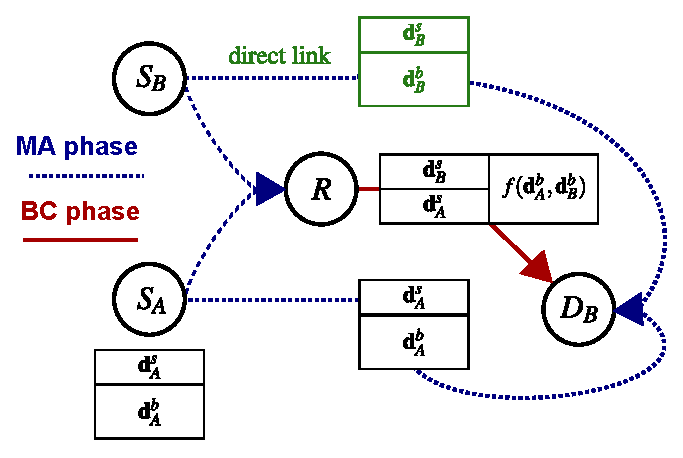
\includegraphics[width=0.75\columnwidth]{fig/2-SRN-sc_principle_BC-TWT_directLink}
\par\end{centering}

\centering{}\caption{Direct channel at destination $D_{B}$ in the robustness analysis
(likewise, a direct channel is assumed to be present also at $D_{A}$).\label{fig:CTUpp_DirectChannel}}
\end{figure}


\begin{figure*}
\centering{\includegraphics[width=1\textwidth]{fig/Robust_20}
\includegraphics[width=1\textwidth]{fig/Robust_21}}
\caption{Robustness analysis for two fixed $(N_{b},N_{s},r_{b},r_{s})$ scenarios.
\label{fig:CTUpp_Robustenss_analysis}}
\end{figure*}

\end{document}
